\section{Homotopy}
\label{sec:Homotopy}

We have already seen homology in chain complexes. We can of course now translate this notion to simplicial abelian groups, by assigning a simplicial abelian group $X$ to $H_n(N(X))$. But there is a more general notion of homotopy for simplicial sets, which is also similar to the notion of homotopy in topology. We will define the notion of homotopy groups for simplicial sets.

When dealing with homotopy groups in a topological space $X$ we always need a base-point $\ast \in X$. This is also the case for simplicial sets. We will notate the chosen base-point of a simplicial set $X$ with $\ast \in X_0$. Note that it is a $0$-simplex, but in fact the base-point is present in all sets $X_n$, because we can consider its degenerate simplices $s_0(\ldots(s_0(\ast))\ldots) \in X_n$, we will also denote these elements as $\ast$. Of course in our situation we are concerned with simplicial abelian groups, where there is an obvious choice for the base-point given by the neutral element $0$.

\subsection{Homotopy groups}
\begin{definition}
	Given a simplicial set $X$ with base-point $\ast$, we define $Z_n(X)$ to be the set of $n$-simplices with the base-point as boundary, i.e.
	$$ Z_n(X) = \{ x \in X_n | d_i(x) = \ast \text{ for all } i \leq n \}. $$
	For two $n$-simplices $x, x' \in Z_n(X)$, we define $x \sim x'$ if there exists $y \in X_{n+1}$ such that
	\begin{align}
		d_0(y) &= x, \\
		d_1(y) &= x', \\
		d_i(y) &= \ast \text{ for all } i > 1.
	\end{align}
	We will call $y$ the \emph{homotopy} and notate $y: x \sim x'$.
\end{definition}

Of course we would like $\sim$ to be an equivalence relation, however this is not true for all simplicial sets. For example there is in general no reason for symmetry, existence of a $1$-simplex $y$ from $x$ to $x'$ does not give us a $1$-simplex $y'$ from $x'$ to $x$. One can give an precise condition on when it is a equivalence relation, the so called \emph{Kan-condition}. In our case of simplicial abelian groups, however, we can prove directly that $\sim$ is an equivalence relation.

In figure~\ref{fig:simplicial_htp} it is shown why the definition of homotopy makes sense for $n=1$. Two homotopic $1$-simplices from $Z_n(X)$ are depicted in two ways. The first way only shows the structure we have, indicating what the boundaries are (as described by the face maps). In the second figure we collapsed all occurrences of $0$ into a single point. This way of drawing a homotopy should remind the reader of homotopy (between paths) in a topological space.

\begin{figure}[h!]
\begin{subfigure}{.5\textwidth}
  \centering
  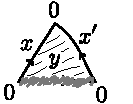
\includegraphics{simplicial_htp1}
\end{subfigure}%
\begin{subfigure}{.5\textwidth}
  \centering
  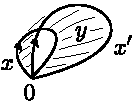
\includegraphics{simplicial_htp2}
\end{subfigure}
\caption{In the figure on the left two homotopic $1$ simplices $x, x' \in Z_n(X)$ are shown. The fact that $d_2(y) = \ast$ is depicted by crossing out the bottom line. The right image shows exactly the same structure if we would draw the $0$-simplex $0$ only once (and hence also collapse the degenerate $1$-simplex $d_2y$).}
\label{fig:simplicial_htp}
\end{figure}

\begin{lemma}
	The relation $\sim$ as defined above is an equivalence relation on $Z_n(X)$. Furthermore it is compatible with addition.
\end{lemma}

Before proving this, one should have a look at figure~\ref{fig:simplicial_eqrel}. In this figure we show what we want to proof in degree $n=0$ (i.e. the simplices of interest are points, and the homotopies are paths).

\begin{figure}[h!]
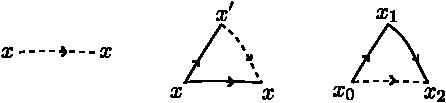
\includegraphics{simplicial_eqrel}
\caption{The three properties of an equivalence relation: reflexivity, symmetry and transitivity. The dashed lines show which homotopy we should construct.}
\label{fig:simplicial_eqrel}
\end{figure}

\begin{proof}
	\emph{Reflexivity}. Let $x \in Z_n(X)$, define $y = s_0 x$. By considering the simplicial identities $d_0 s_0 = \id$ and $d_1 s_0 = \id$, it follows that $d_0 y = d_1 y = x$. Furthermore $d_i y = d_i s_0 x = s_0 d_{i-1} x = 0$ for all $i > 1$, because $x \in Z_n(X)$.

	\emph{Symmetry}. Let $x, x' \in Z_n(X)$ with $y: x \sim x'$. Define $y' = s_0 x + s_0 x' - y$, then by using linearity: $d_0 y' = x + x' - x = x'$ and $d_1 y' = x + x' - x' = x$. For $i>1$ we again get $d_i y' = 0$, because $x \in Z_n(X)$.

	\emph{Transitivity}. Let $x_0, x_1, x_2 \in Z_n(X)$ with $y: x_0 \sim x_1$ and $z: x_1 \sim x_2$. Define $w = y + z - s_0 x_1$. By linearity we have $d_0 w = x_0 + x_1 -x_1 = x_0$, similarly $d_1 w = x_2$. Again for $i>1$ we have $d_i w = 0$.

	\emph{Addition}. Let $y: x_0 \sim x_1$ and $z: x_2 \sim x_3$. Then by linearity $y + z: x_0 + x_2 \sim x_1 + x_3$ and $-y: -x_0 \sim -x_1$.
\end{proof}

\begin{definition}
	Given a simplicial abelian group $X$, we define the $n$-th homotopy group as:
	$$ \pi_n(X) = Z_n(X) / \sim. $$
\end{definition}

Note that this is an abelian group, because $Z_n(X)$ is a subgroup of $X_n$, and $\sim$ also defines a subgroup. It is relatively straight forward to prove that this definition coincides with the $n$-th homology group of the associated normalized chain complex.

\begin{lemma}
	For any simplicial abelian group $X$:
	$$ \pi_n(X) = H_n(N(X)). $$
\end{lemma}
\begin{proof}
	By writing out the definitions of the $n$-cycles and $n$-boundaries of the normalized chain complex, we see:
	\begin{align*}
		\ker(\del) &= \{ x \in N(X)_n \I \del(x) = 0 \} \\
			&= \{ x \in X_n \I d_i(x) = 0 \text{ forall } i > 0 \text{ and } d_0(x) = 0 \} \\
			&= \{ x \in X_n \I d_i(x) = 0 \text{ forall } i \leq n \} \\
			&= Z_n(X) \\
		\im(\del) &= \{ \del(y) \I y \in N(X)_{n+1} \} \\
			&= \{ d_0 y \I y \in X_{n+1}, d_i(y) = 0 \text{ for all } i > 0 \} \\
			&= \{ x \in N(X)_n \I x \sim 0 \}
	\end{align*}
	So we see that $\pi_n(X) = Z_n(X) / \sim = \ker(\del) / \im(\del) = H_n(N(X))$.
\end{proof}

\begin{corollary}
	For a chain complex $C$ we have $H_n(C) \iso \pi_n(K(C))$
\end{corollary}
\begin{proof}
	By the established equivalence we have for any chain complex $C$:
	$$ \pi_n(K(C)) \iso H_n(N(K(C))) \iso H_n(C). $$
\end{proof}

\subsection{Topology}
In Section~\ref{sec:Constructions} we saw that we can construct a functor $G: \cat{C} \to \sSet$ if we are provided a functor the other way around. If we can define a functor $F: \DELTA \to \Top$, then for any space $X$ we have a simplicial set $\Hom{\Top}{F-}{X}: \DELTA^{op} \to \Set$. In Section~\ref{sec:Chain Complexes}, we already defined the \emph{topological $n$-simplex} $\Delta^n$ and face maps $\delta^i : \Delta^n \mono \Delta^{n+1}$. We can similarly define degeneracy maps $s^i: \Delta^n \to \Delta^{n-1}$ as:
$$ s^i(x_0, \ldots, x_n) = (x_0, \ldots, x_i + x_{i+1}, \ldots, x_n) \in \Delta^{n-1}. $$
The reader is invited to check the cosimplicial identities himself and conclude that we now have a functor $F: \DELTA \to \Top$, and hence we have a functor $S: \Top \to \sSet$ given by:
$$ \text{Sing}(X)_n = \Hom{\Top}{\Delta^n}{X}. $$

Recall construction of the singular chain complex in Section~\ref{sec:Chain Complexes}:
$$ C_n(X) = \Z[\Hom{\cat{Top}}{\Delta^n}{X}]. $$
Where the boundary map was given as an alternating sum. Looking more closely we see that this construction decomposes as:
$$ C: \Top \tot{\text{Sing}} \sSet \tot{\Z} \sAb \tot{M} \Ch{\Ab}, $$
where the last functor is the \emph{unnormalized chain complex}. All the categories involved have a notion of homotopy. In topological spaces this is the known notion where $f, g:X \to Y$ are homotopic if there exists a homotopy $H:I \times X \to Y$ with the appropriate properties. In simplicial sets (or simplicial abelian groups) we only saw the notion of homotopy groups, but there exists a more general notion of homotopy, as discussed in the overview of Friedman \cite{friedman}. And finally in chain complexes we saw homology groups, but this category also has a more general notion of chain homotopy, which can be found in any book on homological algebra such as in the book of Rotman \cite{rotman}.

It is known that for any simplicial abelian group both the normalized and unnormalized chain complex have the same homology groups. More precisely for any simplicial abelian group $X$ we have:
$$ H_n(N(X)) \iso H_n(M(X)) \quad\text{for all } n \in \N. $$
This is for example proven in \cite[Theorem 4.1]{eilenberg}. So this assures that the homology groups of the singular chain complex of a space are really the homotopy groups of the simplicial abelian group which is in the background.
